\documentclass{article}
\usepackage{multicol}
\usepackage{graphicx}% Include figure files
\usepackage{dcolumn}% Align table columns on decimal point
\usepackage{bm}% bold math
\usepackage{hyperref}% add hypertext capabilities
\usepackage{booktabs}
\usepackage{listings}
\usepackage{mathtools}
\usepackage{amsmath}
\renewcommand{\abstractname}{\vspace{-\baselineskip}}
\bibliographystyle{plain}
\usepackage[utf8]{inputenc}
\usepackage{verbatim} %for å inkludere filer med tegn LaTeX ikke liker
\usepackage{mathpazo}
\usepackage{float}
\newcommand\numberthis{\addtocounter{equation}{1}\tag{\theequation}}

\begin{document}

\title{Project 3}
<<<<<<< HEAD
\author{Sebastian Amundsen, Marcus Berget and Andreas Wetzel}



\title{Project 3}
\author{Kandidatnummer}

\date{\today}
=======
\author{Kandidatnummer}
>>>>>>> 7d50c1a0f4dec85c9c0a8ff74d28661abd3f07a7

\maketitle

\begin{abstract}

\end{abstract}

\begin{multicols}{2}

<<<<<<< HEAD

\section{Method}
We assume that the earths orbit around the sun is circular. And from circal motion and Newtons gravitational force we have that
\begin{equation}
    F_G=G\frac{M_EM_{\odot}}{r^2}=\frac{M_Ev^2}{r}
\end{equation}
We now want to show that the velocity, $v$, of the earth can be written as
\begin{align}
    v^2r=GM_{\odot}=4\pi^2\frac{AU^3}{yr^2}
\end{align}
Since we say it is circular orbits  can we use the centripetal force to rewrite equation 2 
\begin{align}
    M_E\omega^2r=G\frac{M_EM_{\odot}}{r^2}
\end{align}
where $\omega^2$ is the angular velocity of the earth. Equation 3 can now be rewritten as 
\begin{align}
    M_E(\frac{2\pi}{P})^2r=G\frac{M_EM_{\odot}}{r^2}\\
\end{align}
Where $P$ is a period of the earth around the sun.
Now can we use Keepler's third law, which says that the square of an orbital period $P^2$ equals the cube of the semi-major axis of its orbiting $a^3$
\begin{align}
    P^2=a^3
\end{align}
Where we substitute the circular radius $r$ with the semi-major axis $a$. 

=======
>>>>>>> 7d50c1a0f4dec85c9c0a8ff74d28661abd3f07a7
\section{Introduction}

Though simulating a solar system is interesting and fun enough on it's own, it is naturally also quite useful for the study of astrodynamics. In addition, being able to simulate a solar system provides a good set of tools applicable to many other scientific areas. These tools include having a good understanding of different numerical integration methods, and being able to write a structured and fast code. In this project we wish to explore a model of our own solar system, beginning with simulating the simple two-body system including the Earth and the Sun. We will use this system to compare two different methods of numerical integration, the forward Euler method and the verlocity Verlet method. This simple system also makes a good testing ground for exploring whether our model is consistent with known physical laws such as energy conservation and Kepler's laws of planetary motion. We will also test the stability of the velocity Verlet method by including Jupiter and playing around with it's mass. From there we will include the rest of the planets in our solar system, and blah blah blag general relativity. 

\section{Theory}
<<<<<<< HEAD

=======
>>>>>>> 7d50c1a0f4dec85c9c0a8ff74d28661abd3f07a7

\subsection{Forward Euler}
The forward Euler method is a algorithm to estimate the solution of a differential equation. The Forward Euler method wants to find the next point $\mathbf{r}_{i+1}$. To find the next point, it uses the point it is at, $\mathbf{r}_{n}$, a small time step, $dt$, and the derivative of its position. Which can be expressed like this

\begin{equation}
\mathbf{r}_{n+1}=\mathbf{r}_n + \mathbf{r}_n'\cdot dt
\label{eq:yn1}
\end{equation}

Where $\mathbf{r}_{n+1}$ is the next step, $\mathbf{r}_n$ is the current step, $\mathbf{r}_n'$ is the derived of the current step and $dt$ is the time step.\\
This algorithm is really based abbreviated version of a Taylor expansion, where we only expand the series one step at a time. But by only taking one step at a time, we will also get a local truncation error, which causes an error for each step we take. 

\begin{equation}
\begin{split}
&\mathbf{r}(t_n+dt)=\mathbf{r}_{n+1}\\
&=\mathbf{r}(t_n)+dt\bigg(\mathbf{r}'(t_n) + \frac{\mathbf{r}''(t_n}{2!}dt\\
&+ ... + \frac{\mathbf{r}^p(t_n)}{p!}dt^{p-1}\bigg) + O(dt^{p+1})
\end{split}
\label{eq:ytndt}
\end{equation} 

<<<<<<< HEAD
Where $O(dt^2)$ is the local truncation error. Since the Forward Euler method is a first-order method, will the local truncation error be proportional to the square of the step size. \\
In our case $\mathbf{r}(t_n) \rightarrow \mathbf{r}_n$ is the position, $\mathbf{r}'(t_n)=\mathbf{v}(t_n) \rightarrow \mathbf{r}'_n=\mathbf{v}_n$ is the velocity and $\mathbf{v}(t_n)=\mathbf{a}(t_n,r_n) \rightarrow \mathbf{v}_n=\mathbf{a}_n$ is the acceleration.\\
The update of our position and velocity with a  time step is then given as  
\begin{align}
    \mathbf{r}(t_{n+1})&=\mathbf{r}(t_n) + \mathbf{v}(t_n)dt + O(dt^2)\\
    \mathbf{r}_{n+1}&=r_{n} + v_{n}dt + O(dt^2)\\
    \mathbf{v}(t_{n+1})&=\mathbf{v}(t_n)+\mathbf{a}_ndt + O(dt^2)\\
    \mathbf{v}_{n+1}&=\mathbf{v}_n +\mathbf{a}_n dt + O(dt^2)
\end{align}
Hence, will forward Euler algorithm look like this
\begin{align}
    \mathbf{r}_{n+1}&=\mathbf{r}_n+\mathbf{v}_ndt\\
    \mathbf{v}_{n+1}&=\mathbf{v}_n+\mathbf{a}_ndt\\
    t_{n+1}&=t_n + dt
\end{align}
The number of FLOPS in the Forward Euler method will be 4 FLOPS for each time step, when we look at the addition and multiplication for this algorithm. Since the loop is looping over N times will the number of FLOPS be $4N$. \\
There is also important to notice since the forward Euler method updates the position before the velocity leads to the energy not being conserved
\subsection{Velocity Verlet}

The velocity Verlet is based on the kinematic equations for an moving object, which in our case is the earth's orbit around the sun. If we want to find the next time step for the velocity and position we do a approximation and uses Taylor-expansion.    
=======
Where $R(dt^2)$ is the local truncation error. Since the Forward Euler method is a first-order method, will the local truncation error be proportional to the square of the step size. 

\subsection{Velocity Verlet method}

The velocity Verlet method is based on the kinematic equations for an moving object, which in our case is the earth's orbit around the sun. If we want to find the next time step for the velocity and position we do a approximation and uses Taylor-expansion   

\begin{equation}
v_{t+dt}=v_t +\frac{dt}{2}(\frac{F_t}{m}+\frac{F_{t+m}}{m}) R(dt^3)
\label{eq:steps}
\end{equation}


We can also split the equation above and perform the calculation in several steps like this:

\begin{equation*}
\begin{split}
&v(t+\frac{1}{2}\Delta t)=v(t)+\frac{1}{2}a(t)\Delta t\\
&x(t+\Delta t)=x(t)+v(t+\frac{1}{2}\Delta t)\Delta t\\
&a(t+\Delta t)=f(x(t+\Delta t))\\
&v(t+\Delta t)=v(t+\frac{1}{2}\Delta t)+\frac{1}{2}a(t+\Delta t)\Delta t
\end{split}
\label{eq:steps}
\end{equation*}
>>>>>>> 7d50c1a0f4dec85c9c0a8ff74d28661abd3f07a7

\begin{align}
\mathbf{r}(t\pm dt)&=\mathbf{r}(t)\pm \mathbf{r}'(t)dt + \frac{\mathbf{r}''(t)}{2}dt\\ + O(dt^3)
\end{align}\\
This gives us the position and velocity 
\begin{align}
    \mathbf{r}_{n+1}&=r_n+v_ndt + \frac{\mathbf{a}_n}{2}dt^2+O(dt^3)\\
    \mathbf{v}_{n+1}&=\mathbf{v}_n+\mathbf{a}_ndt+\frac{\mathbf{v}''_n}{2}dt^2 + O(dt^3)
\end{align}
We rewrite expression 19 to define $\mathbf{v}''_n$, we do this by by defining the next step in acceleration $\mathbf{a}_{n+1}=\mathbf{v}'_n$ 
\begin{align}
    \mathbf{a}_{n+1}=\mathbf{v}'_{n+1}=\mathbf{v}'_n+\mathbf{v}''_ndt + O(h^2)
\end{align}
\begin{align}
        \mathbf{v}''_n=\frac{\mathbf{v}'_{n+1}-\mathbf{v_n}}{dt}\\
    =\frac{\mathbf{a}_{n+1}-\mathbf{a}_n}{dt}
\end{align}
Plugging equation 22 into 19 we get the general algorithm for Velocity Verlet. 
\begin{align}
    \mathbf{r}_{n+1}&=\mathbf{r}_n+\mathbf{v}_ndt+\frac{\mathbf{a}_n}{2}dt^2+O(dt^2)\\
    \mathbf{v}_{n+1}&=\mathbf{v}_n+\frac{\mathbf{a}_{n+1}-\mathbf{a}_n}{2}dt+O(dt^3)
\end{align}
\\
\subsection{Conservation of angular momentum}
<<<<<<< HEAD
The definition of Keeplers law is that a area, where a connecting line between a planet and the sun, is always the same for an equal time interval. Which is illustrated in the figure below:


=======
The definition of Keeplers law is that a area, where a connecting line between a planet and the sun, is always the same for an equal time interval. Which is illustrated in the figure below.

>>>>>>> 7d50c1a0f4dec85c9c0a8ff74d28661abd3f07a7
\begin{figure}[H]
	\centering
	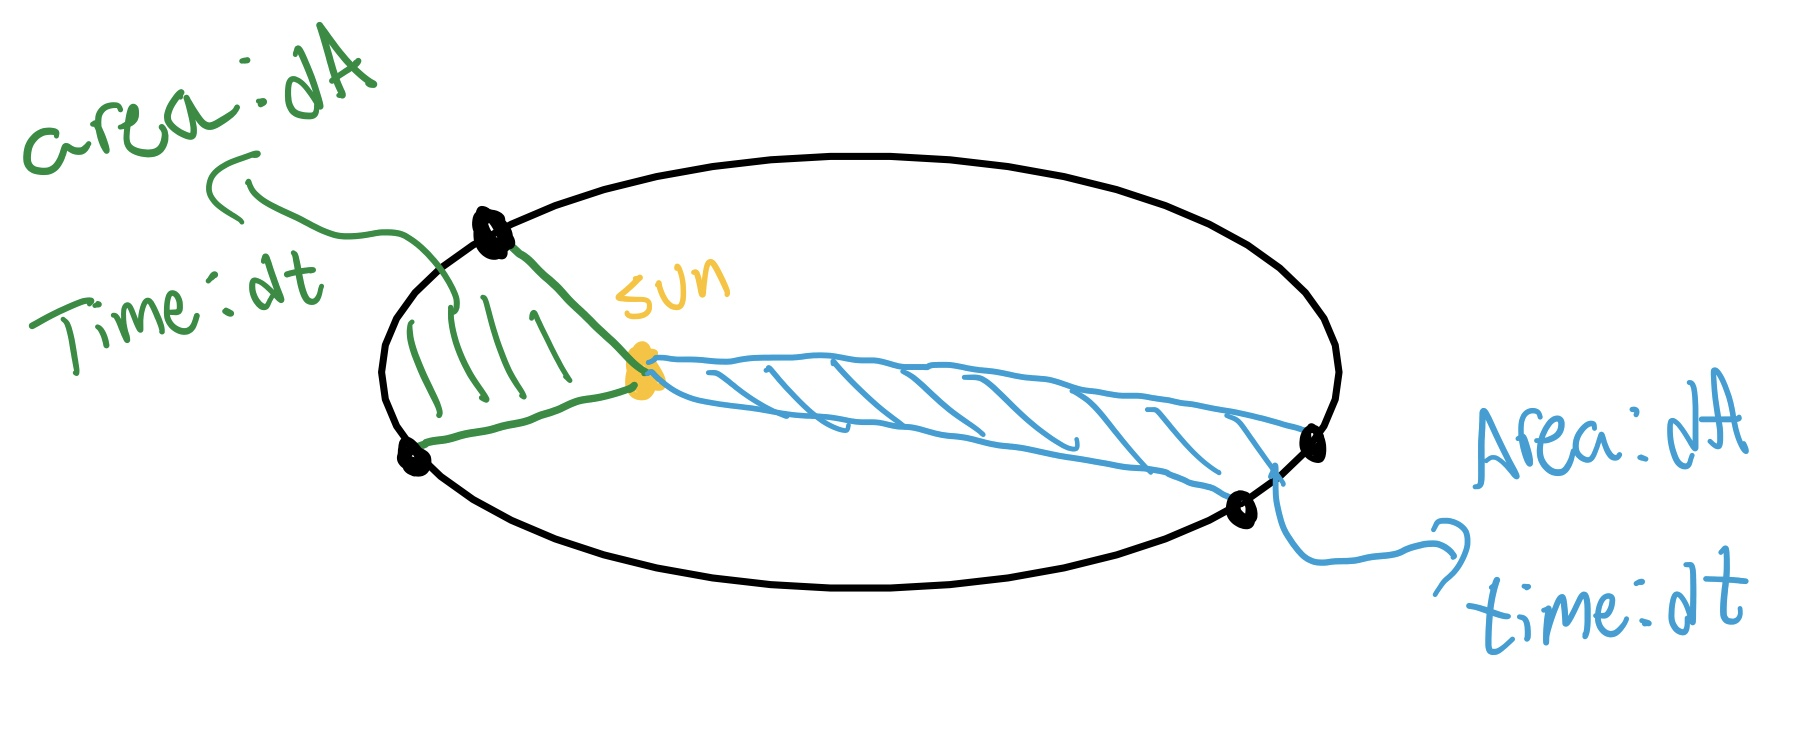
\includegraphics[width=\linewidth]{K2L.jpg}
	\caption{Keeplers second law. Where the area is the same for the same time interval.}
	\label{fig:1bplot}
\end{figure}
<<<<<<< HEAD

The best way to show that the angular momentum is conserved by using Keeplers second law is to make a drawing.

=======
>>>>>>> 7d50c1a0f4dec85c9c0a8ff74d28661abd3f07a7

The best way to show that the angular momentum is conserved by using Keeplers second law is to make a drawing:

\begin{figure}[H]
	\centering
	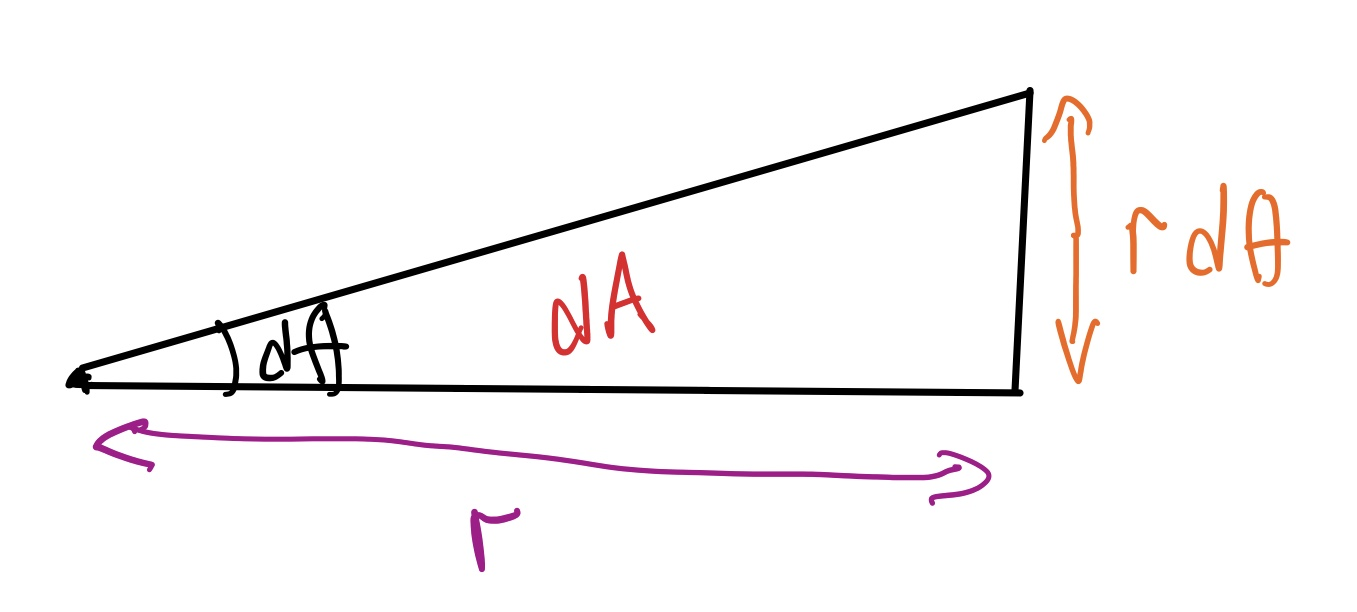
\includegraphics[width=\linewidth]{sketch.jpg}
	\caption{This square is the infinitesimal area dA that the planet has moved by a infinitesimal time interval dt}
	\label{fig:1bplot}
\end{figure}
<<<<<<< HEAD
Figure 2 shows us that the area is 
\begin{align}
=======


Figure 2 shows us that the area is:

\begin{equation}
>>>>>>> 7d50c1a0f4dec85c9c0a8ff74d28661abd3f07a7
    dA=\frac{1}{2}r^2d\theta
\end{align}
We now want to find an infinitesimal area where the planet has moved around the sun, over an infinitesimal time step, where we use equation 12.
\begin{align}
    \frac{dA}{dt}&=\frac{1}2{r^2}\frac{d\theta}{dt}\\
    &=\frac{1}{2}rv_\theta
\end{align}
And the definition of angular momentum is given as
\begin{align}
    L=mrv_\theta
\end{align}
With equation 14 and 15 we can show that the angular momentum is conserved.
\subsection{Testing forms of the force}
Until now we have looked at the movement for the planet with the gravitational force with the square of r. We will now try to change the gravitational force where the power of r is in the range $\beta in [2,3]$ The gravitational force is then given as
\begin{align}
    \mathbf{F}_G=-\frac{GM_{\odot}M_{planet}}{r^{\beta}}\frac{\mathbf{r}}{r}
\end{align}
\subsection{Escape velocity}
We will now look at a planet which begins at a distance 1 AU from the sun, 
and see how fast the initial velocity must be for the planet to be able to escape the sun. We find the analytical solution to compare it to our numerical solution. \\
The analytical expression is given as 
\begin{align}
    \mid{\mathbf{V}_{esc}}\mid=\sqrt{\frac{2GM_{\odot}}{r}}
\end{align}
By plugging equation 2 into 16, and use that our initial position of the planet is $r=AU$ we get
\begin{align}
\mid{\mathbf{V}_{esc}^2}\mid&=\frac{2\cdot 4\pi^2AU^3}{yr^2}\cdot\frac{1}{r}\\
&=\frac{2\cdot 4\pi^2AU^3}{yr^2}\cdot\frac{1}{AU}\\
\mid{\mathbf{V}_{esc}}\mid&=2\sqrt{2}\pi\cdot\frac{AU}{yr}
\end{align}
\subsection{Perihelion precision}
The definition of perihelion precision is that the perihelion point of an objects, in our case Mercury, changes its position because of 
the gravitational field deflection from light. RIKTIG? It is measured to change   
\section{Results}
\subsection{Conservation of angular momentum}
If we substitute equation 15 into equation 14 
\begin{align}
    \frac{dA}{dt}=\frac{1}{2}\frac{L}{m}
\end{align}
Sine $\frac{dA}{dt}$=constant and the mass m is constant means that the angular momentum also is constant and therefore also conserved.  
\end{multicols}



\clearpage
\appendix % Her kommer appendix.
\section{Calculations} 

\bibliography{References} % Kilder.
\begin{thebibliography}{9}
\bibitem{94}
	Skriv inn kilde her.
\end{thebibliography}
<<<<<<< HEAD
=======

>>>>>>> 7d50c1a0f4dec85c9c0a8ff74d28661abd3f07a7
\end{document}
